\chapter{Solution Approach} \label{cha:solution-approach}

We are now going to use the theory discussed in Chapter \ref{cha:fundamentals} to estimate uni- and bivariate  functions using data and a priori domain knowledge. An overview of the different problems considered in this chapter is given in Table \ref{tab:problem_overview}. 

\begin{table}[H]
	\centering
	\begin{tabular}{|l|l|l|l|}
		\hline
		\textbf{Univariate}   & \textbf{Section} & \textbf{Bivariate}         & \textbf{Section} \\ \hline \toprule
		B-splines             &                & Tensor-product B-splines   &               \\ \hline
		P-splines             &                & Tensor-product P-splines   &              \\ \hline
		SCP-splines           & 			   & Tensor-product SCP-splines &     \\ \hline \bottomrule
	\end{tabular}
	\caption{Problem overview.}
	\label{tab:problem_overview}
\end{table}
%
First, we are using B-splines, see Section~\ref{subsec:b-splines}, for the estimation of the unknown function $y = f(x)$, i.e. we solve the optimization problem
\begin{align} \label{eq:OF-B-splines}
	\arg \min_{\vec{\beta}} Q_1(\vec{y}, \vec{\beta}) = \lVert \vec{y} - \vec{X} \vec{\beta} \rVert,
\end{align}
%
using the B-spline or tensor-product B-spline basis matrix $\vec{X}$. Next, we use the concept of P-splines, see Section~\ref{subsec:p-splines}, to estimate smooth functions, i.e. we solve the optimization problem
\begin{align} \label{eq:OF-P-splines}
	\arg \min_{\vec{\beta}} Q_2(\vec{y}, \vec{\beta}; \lambda) = \lVert \vec{y} - \vec{X} \vec{\beta} \rVert + \lambda \cdot \text{pen}(\vec{\beta})
\end{align}
%
where $\text{pen}(\vec{\beta})$ specifies a smoothness penalty term. Finally, we are going to incorporate a priori domain knowledge into the fitting process using shape-constrained P-splines (SCP-splines), i.e. we solve the optimization problem
\begin{align} \label{eq:OF-SCP-splines}
	\arg \min_{\vec{\beta}} Q_3(\vec{y}, \vec{\beta}; \lambda, \lambda_c) = \lVert \vec{y} - \vec{X} \vec{\beta} \rVert + \lambda \cdot \text{pen}(\vec{\beta}) + \lambda_c \cdot \text{con}(\vec{\beta}),
\end{align}
%
where $\text{con}({\vec{\beta}})$ specifies the user-defined shape constraint to incorporate a priori domain knowledge with, see \cite{hofner2011monotonicity} and \cite{bollaerts2006simple}. Various types a priori domain knowledge can be incorporated using the constraints listed in Table~\ref{tab:constraint_overview}.

\begin{table}[H]
	\centering
	\begin{tabular}{|l|ll|l|}
		\hline
		\textbf{Constraint}& & \textbf{Description}   & \textbf{Section}     \\ \hline \toprule
		Jamming            & & $f(x^{(M)}) \approx y^{(M)}$ &	12 \\ \hline 
		\multirow{2}{*}{Boundedness}  & lower & $f(x)\ge M$ 	  &	12 \\ \cline{2-4}
									  & upper & $f(x)\le M$    & 12 \\ \hline
		\multirow{2}{*}{Monotonicity} & increasing & $f'(x) \ge 0$ 	& 23 \\ \cline{2-4}
		& decreasing & $f'(x) \le 0$  & 23 \\ \hline	
		\multirow{2}{*}{Curvature}    & convex     & $f''(x)\ge 0$ 	& 33 \\ \cline{2-4}
		& concave    & $f''(x)\le 0$ 	& 33 \\ \hline
		\multirow{6}{*}{Unimodality}  & \multirow[t]{3}{*}{peak}  & $m = \arg \max_{x} f(x)$  & 44 \\ 
		&	                       & $f'(x) \ge 0 \quad \text{if} \ x < m$ & \\ 
		&  				       & $f'(x) \le 0 \quad \text{if} \ x > m$ & \\ \cline{2-4} 
		& \multirow[t]{3}{*}{valley}& $m = \arg \min_{x} f(x)$  & 44 \\ 
		&	                       & $f'(x) \le 0 \quad \text{if} \ x < m$ & \\ 
		&  				       & $f'(x) \ge 0 \quad \text{if} \ x > m$ &  \\ \hline		\bottomrule
	\end{tabular}
	\caption{Overview of the considered constraints}
	\label{tab:constraint_overview}
\end{table}

The focus of this chapter is the definition and use of shape-constraint P-splines, which are characterize by their parametes $\vec{\beta}$ given by solving the optimization problem~\ref{eq:OF-SCP-splines}.

\section{Shape-constraint P-splines}

In Section~\ref{subsec:p-splines}, we enforced smoothness by penalizing the second-order derivative of the underlying B-spline over the whole input space to create the so-called P-splines.  



\section{Univariate Function Approximation}

\section{Bivariate Function Approximation}
To test the methods listed in the column $\textbf{Univariate}$ in Table~\ref{tab:problem_overview} and the incorporation of a priori domain knowledge, we use the data

\begin{align} \label{eq:dataset-univariate}
	D_{univariate} = \{(x^{(i)}, y^{(i)}), i=1,2,...n\},
\end{align}
%
generated by random sampling of the univariate function $f_1(x)$ given by 

\begin{align}\label{eq:test_func}
	f_1(x) = 3\sin(3\pi x) + 17x + 3 + \epsilon \quad \text{for} \ x \in [0,1],
\end{align}
%
where $\epsilon$ is Gaussian noise given by $\mathcal{N}(0, 0.1)$. The data is shown in~\pref{fig:test_func}. 

\begin{figure}[H]
	\centering
	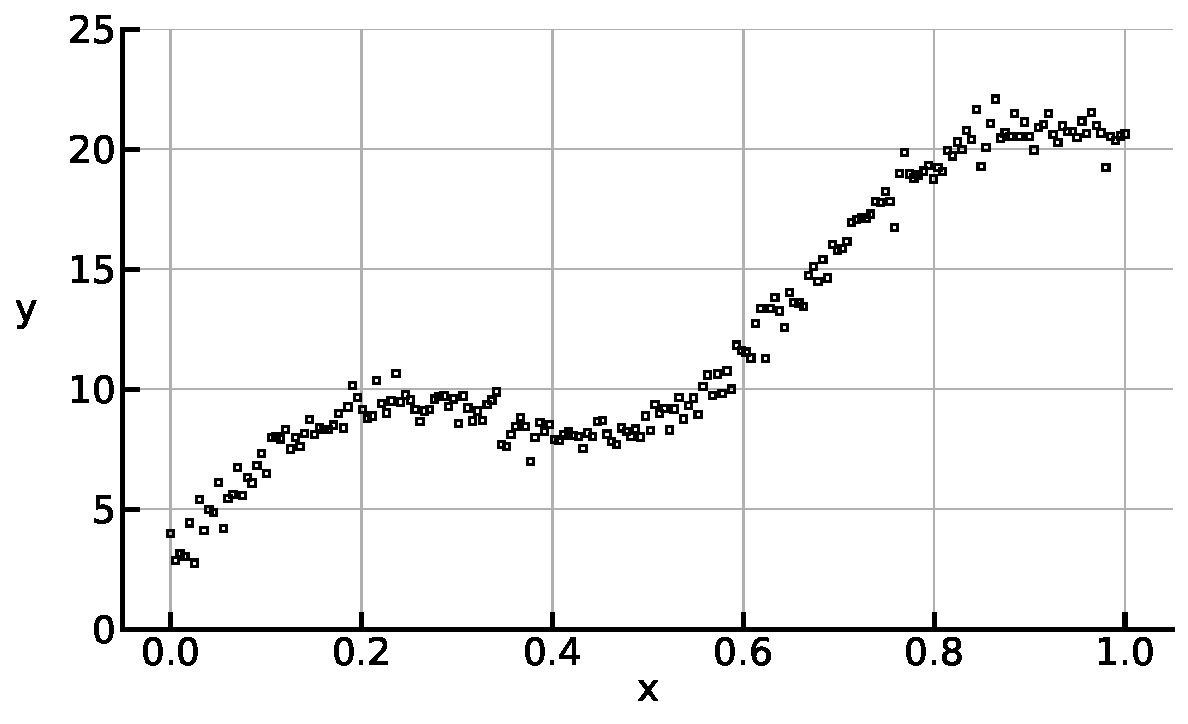
\includegraphics[width=\columnwidth]{thesisplots/test_func.pdf}
	\caption{Noisy samples determined from test function (\ref{fig:test_func})}
	\label{fig:test_func}
\end{figure}

%%%%%%%%%%%%%%%%%%%%%%%%%%%%%%%%%%%%%%%%%%%%%%%%%%%%%%%%%%%%%%%%%%%%%%%%%%%%%%%%%%%%%%%%%%%%%%%%%%%%%%%%%%%%%%%%%


\subsection{1d Function Estimation} \label{subsec:1d-function-estimation}

The goal is to model given data

\begin{align} \label{eq:data}
	\{\vec{x}, \vec{y}\} = \{x^{(i)}, y^{(i)}\}, \ i=1, 2, \dots, n 
\end{align}

using B-splines as basis functions. Therefore, we want to estimate the unknown function $\vec{y} = f(\vec{x})$, which can be represented as a linear combination of $k$ B-spline basis functions $B_j^m$ of degree $m=3$, cf. (\ref{eq:bspline-bf-approach}), as

\begin{align} \label{eq:basis_function_approach}
	\vec{y} = \vec{X} \vec{\beta},
\end{align}

where $\vec{X} \in \mathbb{R}^{n\times k}$ is the B-spline basis matrix, cf. (\ref{eq:bspline-basis-matrix}), and $\vec{\beta} \in \mathbb{R}^k$ are the coefficients to be estimated. 

The least squares objective function to be minimized using the complete data is then given by

\begin{align} \label{eq:OF_1}
	Q_1(\vec{y}, \vec{\beta}) = \lVert \vec{y} - f(\vec{x}) \rVert^2 = \lVert \vec{y} - \vec{X}\vec{\beta} \rVert^2 
\end{align}	

The coefficients are determined ive function $Q_1$ given in (\ref{eq:OF_1}) with respect to $\vec{\beta}$, i.e.

\begin{align}\label{eq:optimization_problem_1}
	\hat{\vec{\beta}}_{LS} = \arg \min_{\vec{\beta}} Q_1(\vec{y}, \vec{\beta}).
\end{align}

Using the least squares algorithm LS, see Chapter \ref{subsubsec:Method-of-LS}, the minimization problem (\ref{eq:optimization_problem_1}) yields 

\begin{align} \label{eq:LS_coef}
	\hat{\vec{\beta}}_{LS}= (\transpose{\vec{X}} \vec{X})^{-1} \transpose{\vec{X}} \vec{y}.
\end{align} 


Figure \ref{fig:smooth_bf} shows a B-spline model using $k=10$ splines on an equidistant grid approximating the noisy data presented in Figure \ref{fig:test_func}, as well as the individual cubic ($m=3$) B-spline basis functions $B_i^3(\vec{x})$ multiplied with the corresponding, estimated coefficients $\hat{\vec{\beta}}_{LS, j} \ j=1, \dots, 10$.

\begin{figure}[H]
	\centering
	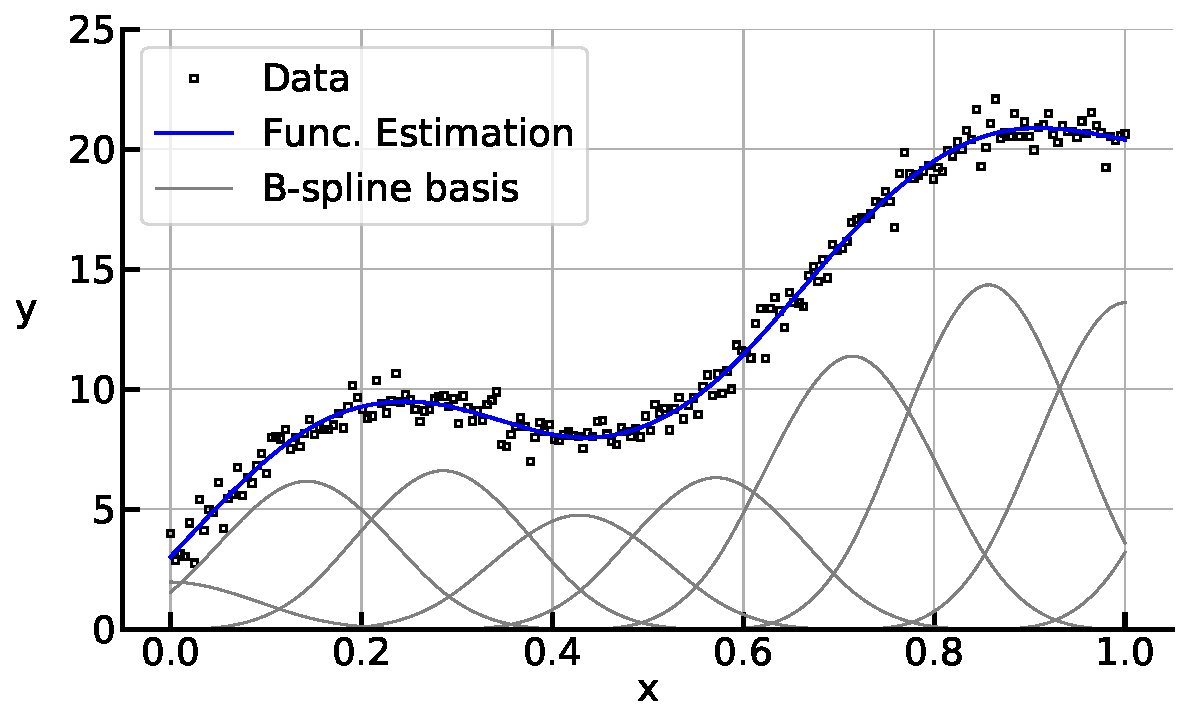
\includegraphics[width=\columnwidth]{thesisplots/smooth_bf.pdf}
	\caption{Approximation of the noisy data by B-splines without constraints}
	\label{fig:smooth_bf}
\end{figure}


Note, the number of splines $k$ has a strong influence on the amount of smoothing. A small number $k$ leads to a very smooth estimate, but a large data error. On the other hand, when the number of splines is relatively large, the data error is very small but the smoothness of the estimate is poor. This behavior is an example of the well-known bias-variance dilemma and depicted in Figure \ref{fig:smooth_bf_large}. \cite{sammut2011}
Here, two B-splines models with $k=10$ and $k=50$ are illustrated, which are applied to the noisy data shown in Figure \ref{fig:test_func}. To overcome this challenges, the B-splines will be extended by penalizing the second derivative of the estimation, see Chapter \ref{subsec:1D_smooth}. 

\begin{figure}[H]
	\centering
	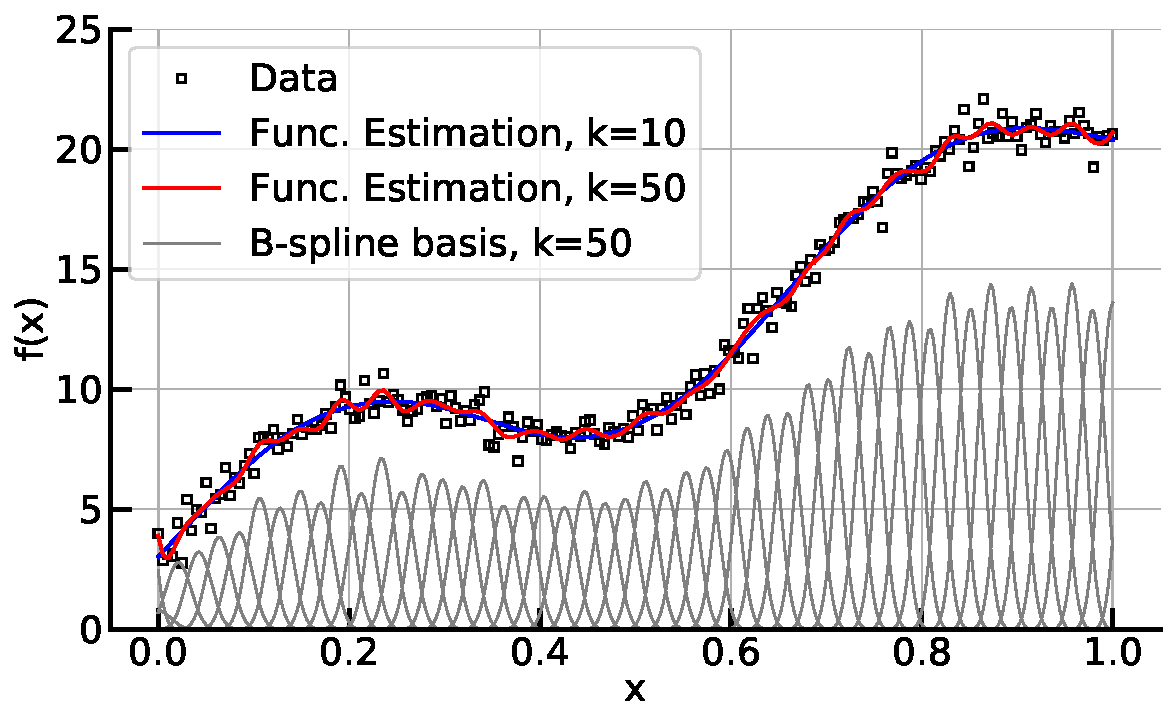
\includegraphics[width=\linewidth]{thesisplots/smooth_wiggly_bf.pdf}
	\caption{Approximation of the noisy data by 10 and 50 B-splines without constraints}
	\label{fig:smooth_bf_large}
\end{figure}


%%%%%%%%%%%%%%%%%%%%%%%%%%%%%%%%%%%%%%%%%%%%%%%%%%%%%%%%%%%%%%%%%%%%%%%%%%%%%%%%%%%%%%%%%%%%%%%%%%%%%%%%%%%%%%%%%
\subsection{1d Smooth Function Estimation} \label{subsec:1D_smooth}

The second derivative of the estimated function $f(x)$, i.e. $f''(x) = \sum_{j=1}^k B''_i(x) \beta_k$, has to be penalized to realize a smoother estimate when using  a high number of splines. Eilers and Marx have introduced the so-called P-splines. \cite{eilers1996flexible}, see Chapter \ref{subsec:p-splines}. Therefore, the objective function in (\ref{eq:OF_1}) is extended by an additional term considering the smoothness, i.e.

\begin{align}\label{eq:OF_2}
	Q_2(\vec{y}, \vec{\beta}) = Q_1(\vec{y}, \vec{\beta}) + \lambda_s \mathcal{J}_s(\vec{\beta}; d) = \lVert \vec{y} - \vec{X} \vec{\beta} \rVert^2 + \lambda_s \transpose{\vec{\beta}} \transpose{\vec{D}}_d \vec{D}_d \vec{\beta}, 
\end{align}

with the smoothing parameter $\lambda_s$ and an appropriate mapping matrix $\vec{D}_d$ capturing the second derivative, which itself is a measure for function wiggliness. Here, an approximation of the second derivative can be performed by the squared finite difference of order $d$ of adjacent coefficients using the matrix form $\vec{D}_d$ of the difference operator of order $d$, see Chapter \ref{subsec:p-splines}. 

By minimizing the objective function (\ref{eq:OF_2}), i.e.

\begin{align}\label{eq:optimization_problem_2}
	\hat{\vec{\beta}}_{PLS} = \arg \min_{\vec{\beta}} Q_2(\vec{y}, \vec{\beta}),
\end{align}

using the penalized least squares algorithm PLS, the penalized least squares estimates are given by

\begin{align} \label{eq:PLS_coef}
	\hat{\vec{\beta}}_{PLS}= (\transpose{\vec{X}} \vec{X} + \lambda_s \transpose{\vec{D}}_d \vec{D}_d)^{-1} \transpose{\vec{X}} \vec{y}.
\end{align} 
%
In (\ref{eq:PLS_coef}), the smoothing parameter $\lambda_s$ plays a critical role and can be optimized using the information criteria specified in Chapter \ref{subsec:MAC}, e.g. AIC and BIC, or by using cross-validation techniques, see Chapter \ref{subsubsec:Cross-validation}. \cite{fahrmeir2007regression}

For small values $\lambda_s \rightarrow 0$, the penalized least squares estimate $\hat{\vec{\beta}}_{PLS}$ approaches the least squares estimate $\hat{\vec{\beta}}_{LS}$, cf. (\ref{eq:LS_coef}), while for large values $\lambda_s \gg 0$, the fitted function shows the behavior of a polynomial with $d-1$ degrees of freedom. For example, using $d=2$ and a large smoothing parameter $\lambda_s$ this configuration leads to a linear function, while using $d=1$ would lead to a constant function. \cite{fahrmeir2007regression}

Figure \ref{fig:psplines} shows the behavior of P-splines of degree $m=3$ using $k=50$ splines for several values of the smoothing parameter $\lambda_s = \{10^{-2}, 10^{2},10^{5},10^{6}\}$ and a smoothness penalty of order $d=2$.  As the value of $\lambda_s$ gets larger, the fitted curve becomes more smooth and thus the $2^{nd}$ derivative of the curve becomes smaller due to the penalty considered in the estimation, see (\ref{eq:PLS_coef}). For very large values of $\lambda_s$, the estimate approaches a straight line, see the yellow curve in Figure \ref{fig:psplines}.

\begin{figure}[H]
	\centering
	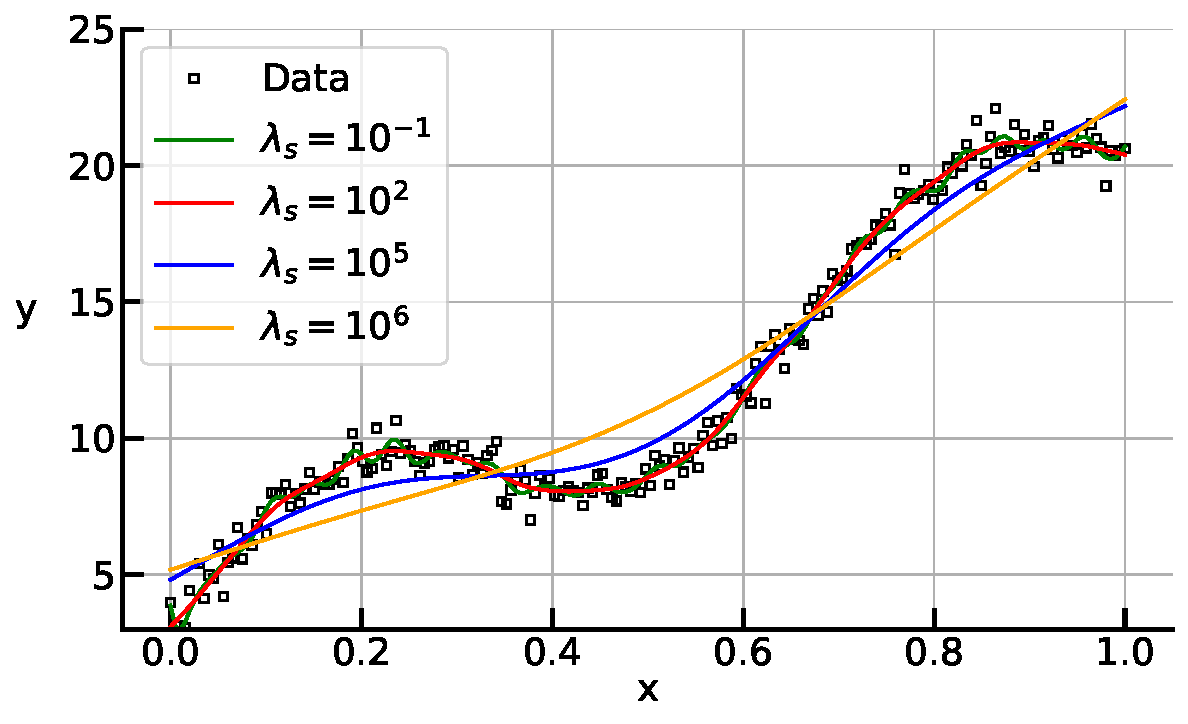
\includegraphics[width=\linewidth]{thesisplots/p_splines.pdf}
	\caption{Smooth function estimation for different smoothing parameters $\lambda_s$}
	\label{fig:psplines}
\end{figure}

%%%%%%%%%%%%%%%%%%%%%%%%%%%%%%%%%%%%%%%%%%%%%%%%%%%%%%%%%%%%%%%%%%%%%%%%%%%%%%%%%%%%%%%%%%%%%%%%%%%%%%%%%%%%%%%%%
\subsection{1d Constraint Function Estimation}

A priori domain knowledge can now be systematically considered by the extension of the objective function (\ref{eq:OF_2}) using an additional term representing the user-defined constraint, see Table \ref{tab:constraint_overview}. Note that this approach incorporates the a priori knowledge as soft constraints. Therefore, no guarantee can be given that the fit holds the constraint for every possible input. The constraint penalized least-squares objective function is given by

\begin{align}\label{eq:OF_3}
	Q_3(\vec{y}, \vec{\beta}) = Q_1(\vec{y}, \vec{\beta}) + \lambda_s \mathcal{J}_s(\vec{\beta}; d) + \lambda_c \mathcal{J}_c(\vec{\beta}; c)
\end{align}

with the corresponding constraint parameter $\lambda_c$, which determines the influence of the user-defined constraint. Note that the parameter $\lambda_c$ has to be set quite large, i.e. $\lambda_c > 10^4$, compared to $\lambda_s$ to enforce the user-defined constraint. 

Constraints for monotonicity, curvature, unimodality, boundedness and jamming can be modeled as 

\begin{align} \label{eq:mapping_matrix}
	\mathcal{J}_c(\vec{\beta}; c) = \transpose{\vec{\beta}} \transpose{\vec{D}}_c \vec{V} \vec{D}_c  \vec{\beta}
\end{align}

with the mapping matrix $\vec{D}_c$ and the diagonal weighting matrix $\vec{V} := \vec{V}(\vec{\beta}; c)$ capturing if the constraint $c$ is active or inactive. The matrices $\vec{D}_c$ and $\vec{V}$ will further be defined in Chapter \ref{sec:user-defined-constraints}.

By minimizing the objective function (\ref{eq:OF_3}), i.e.

\begin{align}\label{eq:optimization_problem_3}
	\hat{\vec{\beta}}_{PLS, c} = \arg \min_{\vec{\beta}} Q_6(\vec{y}, \vec{\beta}),
\end{align}

the constraint penalized least-squares estimate can be given as

\begin{align} \label{eq:PLS,c_coef}
	\hat{\vec{\beta}}_{PLS, c} = (\transpose{\vec{X}} \vec{X} + \lambda_s \transpose{\vec{D}}_d \vec{D}_d + \lambda_c \transpose{\vec{D}}_c \vec{V} \vec{D}_c)^{-1} \transpose{\vec{X}} \vec{y}.
\end{align}	

Note, (\ref{eq:PLS,c_coef}) is a nonlinear equation because the matrix $\vec{V}$ depends on $\vec{\beta}$. Thus, it has to be solved iteratively to calculate optimal coefficients $\hat{\vec{\beta}}_{PLS,c}$. The algorithm is shown in Figure \ref{fig:pirls}. 

\begin{figure}[H]
	\centering
	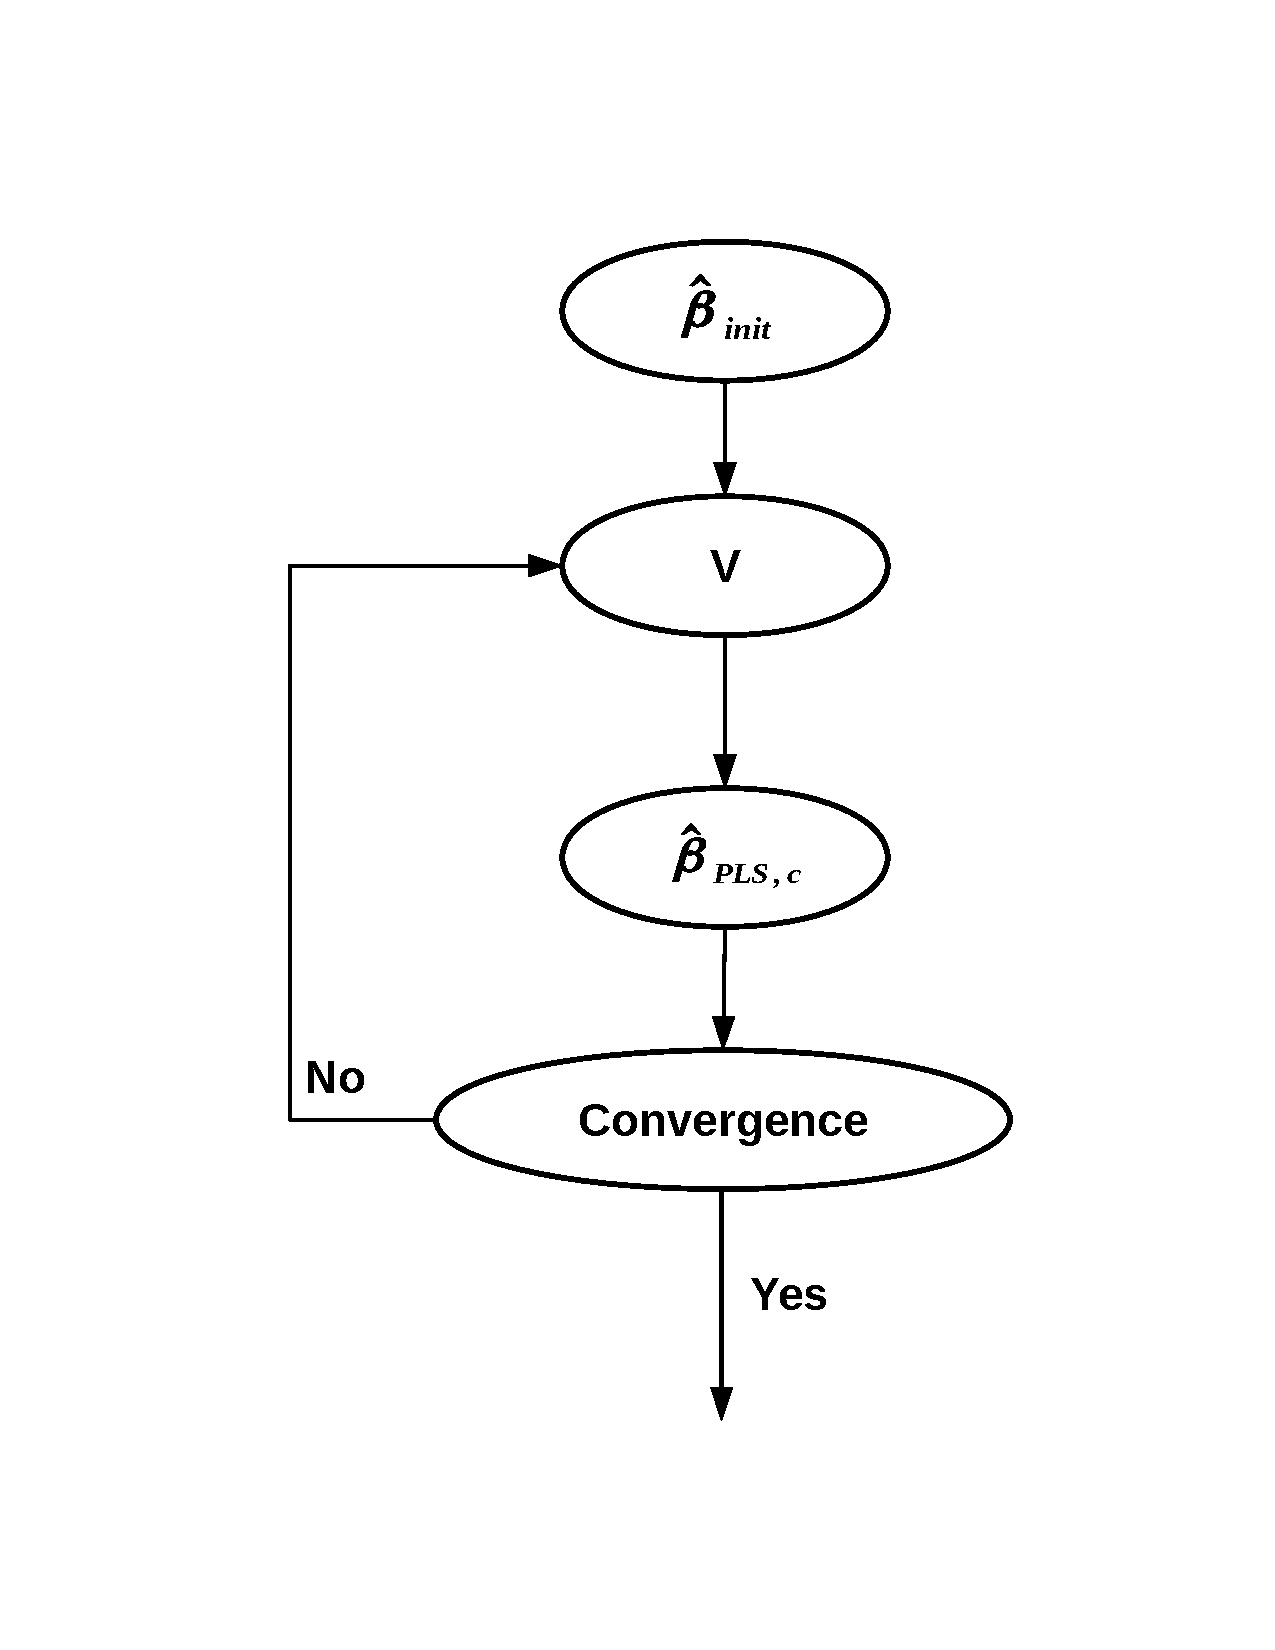
\includegraphics[width=0.6\linewidth]{thesisplots/algorithm.pdf}
	\caption{Penalized iteratively reweighted least squares algorithm}
	\label{fig:pirls}
\end{figure}


The initial estimate $\hat{\vec{\beta}}_{init}$ needed to compute the weighting matrix $\vec{V}$ is given by the least squares estimate $\hat{\vec{\beta}}_{LS}$. Based on the initial estimate $\hat{\vec{\beta}}_{init}$, the weighting matrix $\vec{V}$ and then the constraint least-squares estimate $\hat{\vec{\beta}}_{PLS,c}$ are calculated. The algorithm is performed until no more changes in the weighting matrix $\vec{V}$ appear. This scheme is called the penalized iteratively reweighted least squares and is abbreviated by PIRLS. \cite{hofner2011monotonicity}


Figure \ref{fig:incspline} shows an example, where the noisy data shown in Figure \ref{fig:test_func} is approximated by considering the monotonicity constraint. The estimate has to be monotonically increasing in contrast to the data, i.e. $f'(x) \ge 0$.  The smoothing parameter $\lambda_s$ was optimized using cross-validation and set to $\lambda_s=271.9$. The constraint parameter $\lambda_c$ was set to $\lambda_c = 6000$. For both function estimations, i.e. using P-splines (blue curve) vs. using constraint P-splines (red curve), the number of used splines $k$ was set to $k=30$. 	

\begin{figure}[H]
	\centering
	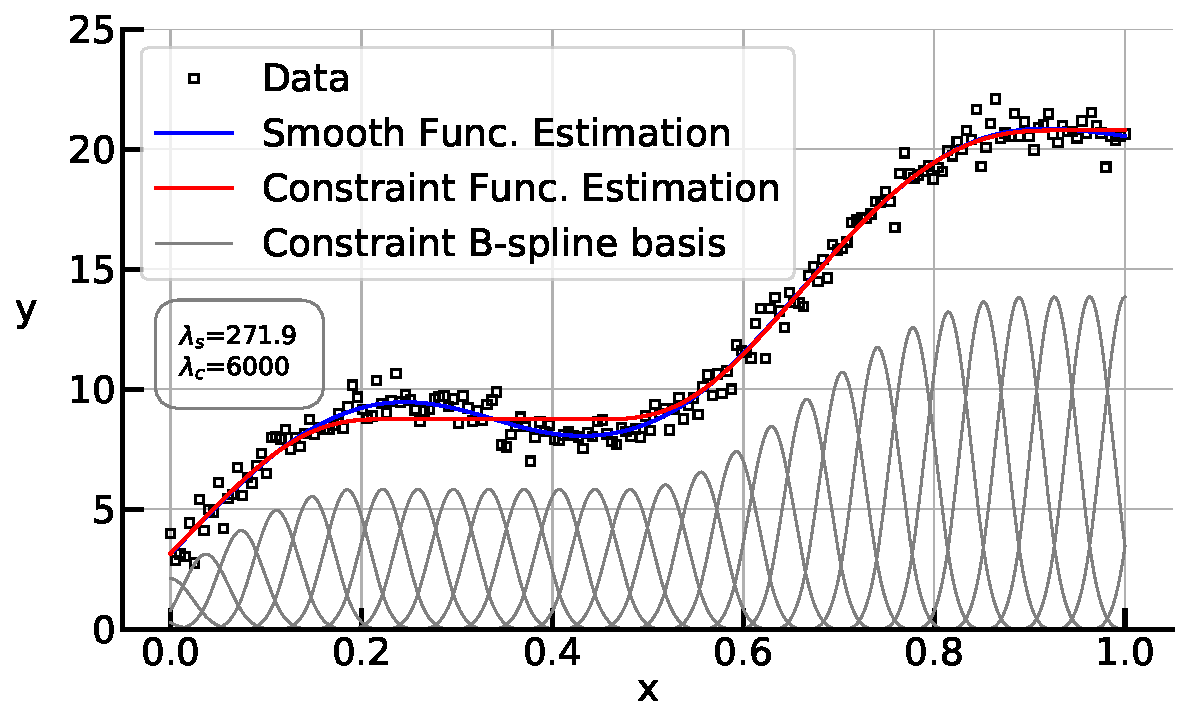
\includegraphics[width=\linewidth]{thesisplots/inc_spline.pdf}
	\caption{Approximation of the noisy data by P-splines and P-splines with the monotonic increasing constraint}
	\label{fig:incspline}
\end{figure}	

The constraint function estimation (red curve in Figure \ref{fig:incspline}), follows the monotonicity constraint far better that the smooth function estimation (blue curve in Figure \ref{fig:incspline}). For $x < 0.15$ and $x > 0.6$, the two fits are nearly identical, since no constraint violation is present. Note, the entries of the weighting matrix $\vec{V}$ in this region are therefore $0$ because the constraint is not active. For $x \in [0.15, 0.6]$ the constraint is active. The red fit produces an almost constant line in this region as an optimal solution for the competing goals of data accuracy, smoothness and constraint fidelity.

This shows, that the incorporation of a priori knowledge in the fitting process using P-splines is in principle possible using an appropriate choice of the mapping matrix $\vec{D}_c$ and the weighting matrix $\vec{V}$ as well as an iterative fitting approach using penalized iteratively reweighted least squares. These matrices are futher discussed in the following chapters.

%%%%%%%%%%%%%%%%%%%%%%%%%%%%%%%%%%%%%%%%%%%%%%%%%%%%%%%%%%%%%%%%%%%%%%%%%%%%%%%%%%%%%%%%%%%%%%%%%%%%%%%%%%%%%%%%%
%%%%%%%%%%%%%%%%%%%%%%%%%%%%%%%%%%%%%%%%%%%%%%%%%%%%%%%%%%%%%%%%%%%%%%%%%%%%%%%%%%%%%%%%%%%%%%%%%%%%%%%%%%%%%%%%%	
\section{User-defined Constraints} \label{sec:user-defined-constraints}

As stated before, a priori domain knowledge given in Table \ref{tab:constraint_overview} can be introduced by the choice of the mapping matrix $\vec{D}_c$ and the weighting matrix $\vec{V}$, cf. (\ref{eq:mapping_matrix}) and (\ref{eq:PLS,c_coef}). Now a description of the different matrices, which are used to enforce the a priori known domain behavior, is presented. 

%%%%%%%%%%%%%%%%%%%%%%%%%%%%%%%%%%%%%%%%%%%%%%%%%%%%%%%%%%%%%%%%%%%%%%%%%%%%%%%%%%%%%%%%%%%%%%%%%%%%%%%%%%%%%%%%%
\subsection{Monotonicity Constraint}

The mapping matrix $\vec{D}_{monoton}$ enforcing monotonic behavior is given by the first order difference operator $\Delta^1$ for equidistant knot placement, cf. \ref{eq:d1-difference-matrix}. The corresponding matrix for $k$ splines is given as

\begin{align} \label{eq:D_c_monoton}
	\vec{D}_{monoton} = \begin{pmatrix}  -1 & 1  &  		& \\ 
		& -1 & 1 		& \\ 
		&    & \ddots  & \ddots  
	\end{pmatrix} \in \mathbb{R}^{k-1 \times k}.
\end{align}

The difference between monotonic increasing and decreasing behavior is controlled by the weighting matrix $\vec{V}$. For increasing behavior, the weighting matrix $\vec{V}$ is given by the weights $v_j$ according to

\begin{align} \label{eq:v_monoton_inc}
	v_j(\vec{\beta}) = \begin{cases}
			0, \quad \text{if} \ \Delta^1\beta_j \ge 0 \\ 
			1, \quad \text{if} \ \Delta^1\beta_j < 0
	\end{cases}	\ \text{for} \ j=2, \dots, k-1.
\end{align}

For decreasing behavior, the weighting matrix $\vec{V}$ is given by the weights $v_j$ according to
\begin{align} \label{eq:v_monoton_dec}
	v_j(\vec{\beta}) = \begin{cases} 0, \quad \text{if} \ \Delta^1\beta_j \le 0 \\ 
		1, \quad \text{if} \ \Delta^1\beta_j > 0
	\end{cases} \ \text{for} \ j=2, \dots, k-1.
\end{align}

This states, that the penalty term $\mathcal{J}_c(\vec{\beta}; c)$ only contributes if adjacent coefficients $\beta_{j-1}$ and $\beta_j$ are increasing or decreasing, respectively. \cite{hofner2011monotonicity} \cite{eilers2005unimodal}

%%%%%%%%%%%%%%%%%%%%%%%%%%%%%%%%%%%%%%%%%%%%%%%%%%%%%%%%%%%%%%%%%%%%%%%%%%%%%%%%%%%%%%%%%%%%%%%%%%%%%%%%%%%%%%%%%	
\subsection{Curvature Constraint}

In the simplest case, the curvature of the function $f(x)$ can either be convex, i.e. $f''(x) \ge 0$, or concave, i.e. $f''(x) \le 0$. The mapping matrix $\vec{D}_{curvature}$ enforcing this behavior can be approximated by the second order difference operator $\Delta^2$ for equidistant knot placement, cf. (\ref{eq:d2-difference-matrix}). The corresponding matrix for $k$ splines is given as

\begin{align} \label{eq:D_c_curvature}
	\vec{D}_{curvature} = \begin{pmatrix} 1 & -2 & 1 		&  		 & \\ 
		& 1  &-2 	    &1 		 & \\
		& 	  & \ddots  & \ddots & \ddots  
	\end{pmatrix} \in \mathbb{R}^{k-2 \times k}.
\end{align}	

The difference between concave and convex curvature is controlled by the weighting matrix $\vec{V}$. For concave curvature, the weighting matrix $\vec{V}$ is given by the weights $v_j$ according to

\begin{align}\label{eq:v_curvature_concave}
	v_j(\vec{\beta}) = \begin{cases} 
		0, \quad \text{if} \ \Delta^2\beta_j \le 0 \\ 
		1, \quad \text{if} \ \Delta^2\beta_j > 0
	\end{cases} \ \text{for} \ j=1, \dots, k-2.
\end{align}

For convex curvature, the weighting matrix $\vec{V}$ is given by the weights $v_j$ according to

\begin{align}\label{eq:v_curvature_convex}
	v_j(\vec{\beta}) = \begin{cases} 
		0, \quad \text{if} \ \Delta^2\beta_j \ge 0 \\ 
		1, \quad \text{if} \ \Delta^2\beta_j < 0
	\end{cases}\ \text{for} \ j=1, \dots, k-2.
\end{align}	

Therefore, the penalty term $\mathcal{J}_c(\vec{\beta}; c)$ in (\ref{eq:OF_3}) or (\ref{eq:PLS,c_coef}) only contributes if the second order difference of adjacent coefficients $\vec{\beta}$ is either positive or negative, respectively. \cite{eilers2005unimodal}

%%%%%%%%%%%%%%%%%%%%%%%%%%%%%%%%%%%%%%%%%%%%%%%%%%%%%%%%%%%%%%%%%%%%%%%%%%%%%%%%%%%%%%%%%%%%%%%%%%%%%%%%%%%%%%%%%	
\subsection{Unimodality Constraint}

We assume that there is a peak in the data $\{x^{(i)}, y^{(i)}\}$ and therefore want to constrain the fit to include a peak. The peak constraint is given by the unimodal mapping matrix $D_{unimodal}$ and the peak weighting matrix $V$. A function $f(x)$ is said to be unimodal if for some value $m$, it is monotonically increasing for $x \le m$ and monotonically decreasing for $x \ge m$. 

The mapping matrix $\vec{D}_{unimodal}$ enforcing unimodal behavior can be constructed using the first order difference operator $\Delta^1$ for equidistant knot placement, cf. (\ref{eq:d1-difference-matrix}), and is given for $k$ splines as 

\begin{align}\label{eq:D_c_unimodal}
	\vec{D}_{unimodal} = \begin{pmatrix} -1 & 1 \\ 
		& \ddots & \ddots  \\
		& & -1 & 1
	\end{pmatrix} \in \mathbb{R}^{k-1 \times k}
\end{align}

The weighting matrix $\vec{V}$ now has a special structure. First, we construct the B-spline basis using the given data as in Chapter \ref{subsec:b-splines}. We then need to find the index $j_{peak}$ of the \emph{peak spline}, which has the maximal value at the peak data point $\max \{f(x^{(i)}) \ \forall \ i \}$, see Figure \ref{fig:peak_spline}. The index $j_{peak}$ is now used as splitting point for the weighting matrix $\vec{V}$. All coefficients $\beta_j$ for $j < j_{peak}$ are constrained to be monotonic increasing, i.e. $\Delta^1 \beta_j \ge 0$ for $j = 1, \dots, j_{peak}-1$, while all coefficients $\beta_j$ for $j > j_{peak}$ are constrained to be monotonic decreasing, i.e. $\Delta^1 \beta_j \le 0$ for $j = j_{peak}+1, \dots, k$. The coefficient $\beta_{j_{peak}}$ stays unconstrained. \cite{eilers2005unimodal} 

\begin{figure}[H]
	\centering
	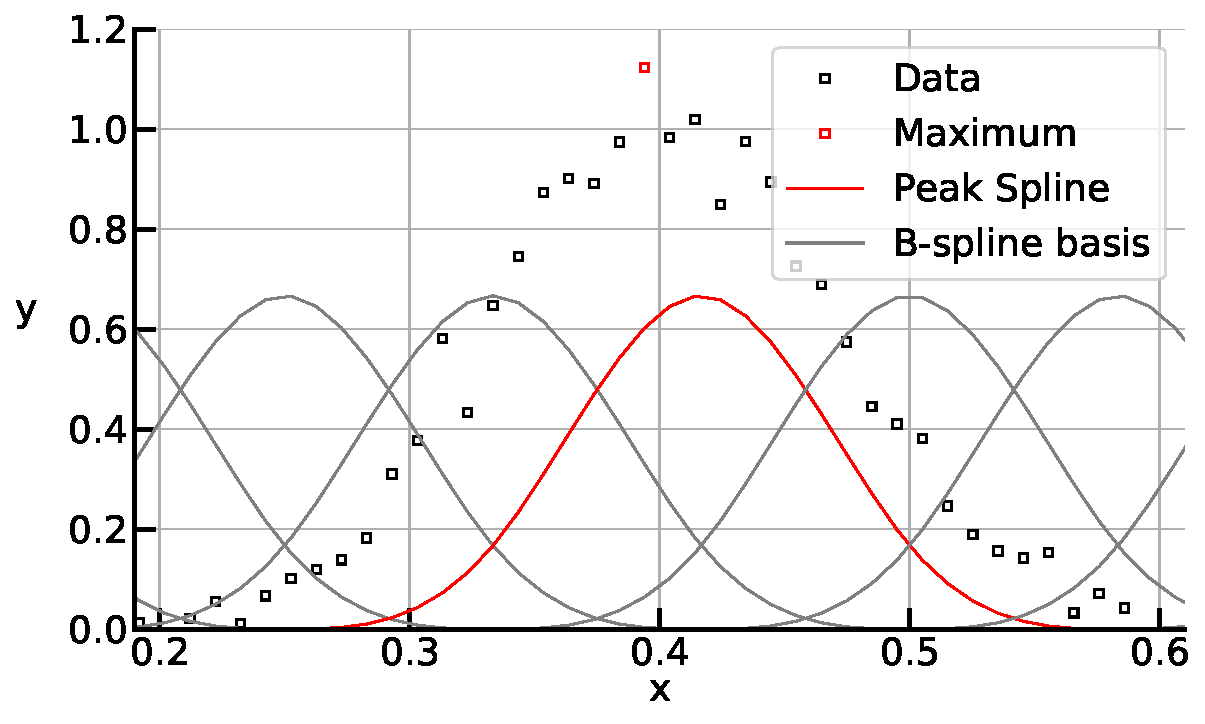
\includegraphics[width=\linewidth]{thesisplots/peak_spline.pdf}
	\caption{Identification of the peak spline based on data}
	\label{fig:peak_spline}
\end{figure}


The weights $v_j$ to incorporate the peak constraint have the following structure, i.e.

\begin{align}\label{eq:v_peak_1}
	v_j(\vec{\beta}) &= \begin{cases} 
		0, \quad \text{if} \ \Delta^1\beta_j \ge 0 \\ 
		1, \quad \text{if} \ \Delta^1\beta_j  < 0
	\end{cases}, \quad \text{for} \ j=2, \dots, j_{peak}-1
\end{align}

and 

\begin{align}\label{eq:v_peak_2}
	v_j(\vec{\beta}) &= \begin{cases} 
		0, \quad \text{if} \ \Delta^1\beta_j \le 0 \\ 
		1, \quad \text{if} \ \Delta^1\beta_j > 0
	\end{cases}, \quad \text{for} \ j=j_{peak}+1, \dots, k.
\end{align}

The weight $v_{j_{peak}}$ for the \emph{peak spline} is given by $v_{j_{peak}}(\vec{\beta}) = 0$. 

When assuming a valley in the data, the same approach as above can easily be used by multiplying the data with $-1$ or by always doing the inverse operation, i.e. finding the index $j_{valley}$ of the \emph{valley spline}, then constraining all splines for $j < j_{valley}$ to be monotonic decreasing, i.e. $\Delta^1 \beta_j \le 0$ for $j = 1, \dots, j_{valley}-1$, and all splines for $j > j_{valley}$ to be monotonic increasing, i.e. $\Delta^1 \beta_j \ge 0$ for $j = j_{valley}+1, \dots, k$. The coefficient $\beta_{j_{valley}}$ stays unconstrained. 

The weights $v_j$ to consider a valley constraint are given by

\begin{align}\label{eq:v_valley_1}
	v_j(\vec{\beta}) &= \begin{cases} 
		0, \quad \text{if} \ \Delta^1\beta_j \le 0 \\ 
		1, \quad \text{if} \ \Delta^1\beta_j > 0
	\end{cases}, \quad \text{for} \ j=2, \dots, j_{valley}-1
\end{align}

and 

\begin{align}\label{eq:v_valley_2}
	v_j(\vec{\beta}) &= \begin{cases} 
		0, \quad \text{if} \ \Delta^1\beta_j \ge 0 \\ 
		1, \quad \text{if} \ \Delta^1\beta_j < 0.
	\end{cases}, \quad \text{for} \  j=j_{valley}+1, \dots, k.
\end{align}

The weight $v_{j_{valley}}$ for the \emph{valley spline} is given by $v_{j_{valley}}(\vec{\beta}) = 0$.

%%%%%%%%%%%%%%%%%%%%%%%%%%%%%%%%%%%%%%%%%%%%%%%%%%%%%%%%%%%%%%%%%%%%%%%%%%%%%%%%%%%%%%%%%%%%%%%%%%%%%%%%%%%%%%%%
\subsection{Boundedness Constraint}

For certain physical systems, it is known a priori that the measured quantity cannot be smaller than zero, i.e. $f(x) \ge 0$. Using data-driven modeling on noisy data can lead to predictions in the interpolation and extrapolation regime, which may not hold this constraint due to uncertainties captured by the data. It is therefore appropriate to apply the user-defined constraint of boundedness from below.

The user-defined constraint for boundedness from below by $M=0$ uses as mapping matrix $\vec{D}_c$ the B-spline basis matrix $\vec{X} \in \mathbb{R}^{n \times k}$. The weighting matrix $\vec{V} \in \mathbb{R}^{n\times n}$, with individual weights $v_j$, is specified as follows:

\begin{align} \label{eq:v_boundedness}
	v_j(\vec{\beta}) = \begin{cases} 
		0, \quad \text{if} \ f(x^{(j)}) \ge M\\ 
		1, \quad \text{if} \ f(x^{(j)})  < M 		
	\end{cases} \text{for} \ j=1, \dots, n.
\end{align}

Using different values of $M$ allows us to bound from below from any number $M$. Switching the comparison operators in (\ref{eq:v_boundedness}) enables us to bound functions from above. 

%%%%%%%%%%%%%%%%%%%%%%%%%%%%%%%%%%%%%%%%%%%%%%%%%%%%%%%%%%%%%%%%%%%%%%%%%%%%%%%%%%%%%%%%%%%%%%%%%%%%%%%%%%%%%%%%
\subsection{Jamming Constraint}

Jamming the function $f(x)$ by some point $p = \{x^{(jamm)}, y^{(jamm)}\}$ means that the estimated function $f(x^{(jamm)}) \approx y^{(jamm)}$. This can be incorporated using the B-spline basis matrix $\vec{X} \in \mathbb{R}^{n \times k}$ as mapping matrix $\vec{D}_c$ and a weighting matrix $\vec{V} \in \mathbb{R}^{n \times n}$ given by

\begin{align} \label{eq:v_jamming}
	v_j(\vec{\beta}) = 
		\begin{cases}
			0, \quad \text{if} \ x^{(j)} \ne x^{(jamm)} \\
			1, \quad \text{if} \ x^{(j)} = x^{(jamm)} 
	\end{cases} \text{for} \ j = 1, \dots, n.
\end{align} 

%%%%%%%%%%%%%%%%%%%%%%%%%%%%%%%%%%%%%%%%%%%%%%%%%%%%%%%%%%%%%%%%%%%%%%%%%%%%%%%%%%%%%%%%%%%%%%%%%%%%%%%%%%%%%%%%
\subsection{Penalty Term for Tensor-Product Splines}

To extend the framework of mapping matrices to two dimensions and tensor-product splines, we again use the concept of Kronecker products given in Chapter \ref{subsubsec:tp-splines}. In principle, every possible pair of one dimensional user-defined constraints can be constructed using the approach in Chapter \ref{subsubsec:tp-splines}, e.g. unimodality in two dimensions would be obtained using the unimodal mapping matrix depicted above for each dimension. We then also need to include the constraint specific weight matrices $\vec{V}$.

The penalty term for the constraint given by $c_1$ for dimension $1$ and $c_2$ for dimension $2$ then has the form

\begin{align} \label{eq:J-c-tps}
	\mathcal{J}_c(\vec{\beta}; c) = \transpose{\vec{\beta}} \Big[ \vec{I}^2 \otimes \vec{K}_{c_1} + \vec{K}_{c_2} \otimes \vec{I}^1\Big] \vec{\beta}
\end{align}

with the respective penalty matrices $\vec{K}_{c_1} = \vec{D}_{c_1}^{\text{T}} \vec{V}_1 \vec{D}_{c_1}$ for dimension $x_1$ and $\vec{K}_{c_2} = \vec{D}_{c_2}^{\text{T}} \vec{V}_2 \vec{D}_{c_2}$ for dimension $x_2$ using the weighting matrices $\vec{V}_1$ and $\vec{V}_2$, the mapping matrices $\vec{D}_{c_1}$ and $\vec{D}_{c_2}$ and the identity matrices $\vec{I}^1$ and $\vec{I}^2$ for the respective dimension.

%%%%%%%%%%%%%%%%%%%%%%%%%%%%%%%%%%%%%%%%%%%%%%%%%%%%%%%%%%%%%%%%%%%%%%%%%%%%%%%%%%%%%%%%%%%%%%%%%%%%%%%%%%%%%%%%%
%%%%%%%%%%%%%%%%%%%%%%%%%%%%%%%%%%%%%%%%%%%%%%%%%%%%%%%%%%%%%%%%%%%%%%%%%%%%%%%%%%%%%%%%%%%%%%%%%%%%%%%%%%%%%%%%%
\section{n-d Constraint Function Estimation}

The extension from one input to multiple input dimensions uses the concept of additive models given in Chapter \ref{subsubsec:STAR}. Given input data $\{ x_1^{(i)}, \dots, x_q^{(i)}, y^{(i)}\}, \ i=1, 2, \dots, n$ and $q$ as the number of inputs, the combined model using all available B-splines and tensor-product splines is given, cf. (\ref{eq:STAR}), as

\begin{align} \label{eq:tps_all}
	y = f(x_1,..., x_q) = \sum_{j=1}^q s_j(x_j) + \sum_{j=1}^{q-1} \sum_{r>j}^q t_{j, r}(x_j, x_r)
\end{align}

where $s_j(x_j)$ is the B-spline estimate given by $s_j(x_j) = \vec{X}_{s_j} \vec{\beta}_{s_j}$ and $t_{j, r}(x_j,x_r)$ is the tensor-product estimate is given by $t_{j, r}(x_j,x_r) = \vec{X}_{t_{j,r}} \vec{\beta}_{t_{j, r}}$. The number of individual estimates is given by 

\begin{align}
	n_{total} = q + \frac{q(q-1)}{2}.  
\end{align}

The constrained penalized least squares objective function for additive models can now be written similar to (\ref{eq:OF_3}) as

\begin{align}\label{eq:OF_6}
	Q_6(\vec{y}, \vec{\beta}) = Q_1(\vec{y}, \vec{\beta}) + \transpose{\vec{\lambda}}_s	\vec{\mathcal{J}}_s(\vec{\beta}; \vec{d}) + \transpose{\vec{\lambda}}_c \vec{\mathcal{J}}_c(\vec{\beta}; \vec{c}).
\end{align}

with $\vec{\lambda}_s \in \mathbb{R}^{n_{total}}$ and  $\vec{\lambda}_c \in \mathbb{R}^{n_{total}}$  defined as vectors with one value of smoothness and constraint parameter for each individual estimate, respectively. 

We now need to specify the three parts of the objective function in (\ref{eq:OF_6}). 

%%%%%%%%%%%%%%%%%%%%%%%%%%%%%%%%%%%%%%%%%%%%%%%%%%%%%%%%%%%%%%%%%%%%%%%%%%%%%%%%%%%%%%%%%%%%%%%%%%%%%%%%%%%%%%%%%
\subsection{Data Term}

Assuming the use of $k$ splines for the B-spline estimates and $k^2$ splines for the tensor-product estimates, the total number of coefficients to be determined is given by 

\begin{align}\label{eq:tps_total_number_of_coef}
	k_{total} = qk + \frac{q(q-1)}{2}k^2. 
\end{align}

Since all B-spline and tensor-product spline models follow a linear model structure, see Chapter \ref{subsec:b-splines} and \ref{subsubsec:tp-splines}, we can combine them into one large model, cf. (\ref{eq:STAR-block-diag}), given by

\begin{align}\label{eq:tps_lin_mod}
	\vec{y} = \vec{X} \vec{\beta}
\end{align}

where the matrix $\vec{X} \in \mathbb{R}^{n \times k_{total}}$ is given in (\ref{eq:STAR-block-diag}) as horizontal concatenation of the individual bases and the combined coefficient vector $\vec{\beta} \in \mathbb{R}^{k_{total}}$ is given in (\ref{eq:STAR-block-diag}) by a vertical concatenation of the individual coefficient vectors. 

The data term $Q_1(\vec{y}, \vec{\beta})$ in the constrained penalized least squares objective function given in (\ref{eq:OF_6}) can now be evaluated using arbitrary input dimensions. 

%%%%%%%%%%%%%%%%%%%%%%%%%%%%%%%%%%%%%%%%%%%%%%%%%%%%%%%%%%%%%%%%%%%%%%%%%%%%%%%%%%%%%%%%%%%%%%%%%%%%%%%%%%%%%%%%%
\subsection{Smoothness Term}

The combined smoothness penalty term $\vec{\mathcal{J}}_s(\vec{\beta}; \vec{d}) \in \mathbb{R}^{n_{total}}$ is then given as

\begin{align}\label{eq:J_s_ndim}
	\vec{\mathcal{J}}_s(\vec{\beta}; \vec{d}) &= 
	\begin{pmatrix}
		\mathcal J_{s_1}(\vec{\beta}_{s_1}; d_{s_1}) \\ 
		\vdots \\ 
		\mathcal J_{s_q}(\vec{\beta}_{s_q}; d_{s_q}) \\
		\mathcal J_{t_{1,2}}(\vec{\beta}_{t_{1,2}}; d_{t_{1,2}}) \\
		\vdots \\
		\mathcal J_{t_{q-1,q}}(\vec{\beta}_{t_{q-1,q}}; d_{t_{q-1,q}}) \\
	\end{pmatrix}
\end{align}

with $\mathcal J_e(\vec{\beta}_e; d_e) = \transpose{\vec{\beta}}_e \transpose{\vec{D}}_{d_e} \vec{D}_{d_e} \vec{\beta}_e$ determining the smoothness penalty term using the coefficients $\vec{\beta}_e$ and mapping matrix $\vec{D}_{d_e}$, see Chapter \ref{subsec:p-splines} and Chapter \ref{subsubsec:tp-splines}, for each estimate $e \in \{s_1, \dots, s_q, t_{1,2}, \dots, t_{q-1,q}\}$. The vector $\vec{d} \in \mathbb{R}^{n_{total}}$ consists of the orders $d_e$ determining the mapping matrix $\vec{D}_{d_e}$ of the smoothness constraint for each individual estimate $e$. 

%%%%%%%%%%%%%%%%%%%%%%%%%%%%%%%%%%%%%%%%%%%%%%%%%%%%%%%%%%%%%%%%%%%%%%%%%%%%%%%%%%%%%%%%%%%%%%%%%%%%%%%%%%%%%%%%%
\subsection{Constraint Term}
The combined constraint penalty term $\vec{\mathcal{J}}_c(\vec{\beta}; \vec{c}) \in \mathbb{R}^{n_{total}}$ is then given as

\begin{align}\label{eq:J_c_ndim}
	\vec{\mathcal{J}}_c(\vec{\beta}; \vec{c}) &= 
	\begin{pmatrix}
		\mathcal J_{s_1}(\vec{\beta}_{s_1}; c_{s_1}) \\ 
		\vdots \\ 
		\mathcal J_{s_q}(\vec{\beta}_{s_q}; c_{s_q}) \\
		\mathcal J_{t_{1,2}}(\vec{\beta}_{t_{1,2}}; c_{t_{1,2}}) \\
		\vdots \\
		\mathcal J_{t_{q-1,q}}(\vec{\beta}_{t_{q-1,q}}; c_{t_{q-1,q}}) \\
	\end{pmatrix}
\end{align}

with $\mathcal J_e(\vec{\beta}_e; c_e) = \transpose{\vec{\beta}}_e \transpose{\vec{D}}_{c_e} \vec{V}_{c_e} \vec{D}_{c_e} \vec{\beta}_e$ determining the constraint penalty term using the coefficients $\vec{\beta}_e$, the mapping matrix $\vec{D}_{c_e}$ and the weighting matrix $\vec{V}_e$ for each estimate $e \in \{s_1, \dots, s_q, t_{1,2}, \dots, t_{q-1,q}\}$, see Chapter (\ref{sec:user-defined-constraints}). The vector $\vec{c} \in \mathbb{R}^{n_{total}}$ consists of the constraint type $c_e$, e.g. monoton increasing, determining the mapping matrix $\vec{D}_{c_e}$ for each individual estimate $e$. 

%%%%%%%%%%%%%%%%%%%%%%%%%%%%%%%%%%%%%%%%%%%%%%%%%%%%%%%%%%%%%%%%%%%%%%%%%%%%%%%%%%%%%%%%%%%%%%%%%%%%%%%%%%%%%%%%%

The objective function (\ref{eq:OF_6}) is then optimized, i.e.

\begin{align}\label{eq:optimization_problem_6}
	\hat{\vec{\beta}}_{PLS,c,nd} = \arg \min_{\vec{\beta}} Q_6(\vec{y}, \vec{\beta}),
\end{align}

using the penalized iteratively reweighted least squares algorithm, cf. (\ref{eq:PLS,c_coef}), to obtain the coefficients $\hat{\vec{\beta}}_{PLS,c,nd}$ as

\begin{align} \label{eq:beta-pls-c-nd-formula}
	\hat{\vec{\beta}}_{PLS,c,nd} = (\transpose{\vec{X}} \vec{X} +\vec{K}_s + \vec{K}_c)^{-1} \transpose{\vec{X}} \vec{y}. 
\end{align}

In (\ref{eq:beta-pls-c-nd-formula}), $\vec{X} \in \mathbb{R}^{n \times k_{total}}$ is the combined basis matrix, cf. (\ref{eq:STAR-block-diag}), $\vec{K}_s \in \mathbb{R}^{k_{total} \times k_{total}}$ is the combined smoothness matrix given as

\begin{align} \label{eq:combined-smoothness-matrix}
	\vec{K}_s = \rotatebox{-90}{$\begin{pmatrix} 
					\lambda_{s_1} \transpose{\vec{D}_{d_{s_1}}} \vec{D}_{d_{s_1}} & 0 \\
					 							0 						  &	\ddots & 0 \\
					 													  &  0 	   & \lambda_{s_q} \transpose{\vec{D}_{d_{s_q}}} \vec{D}_{d_{s_q}} & 0 \\
					 													  &        &           0										   & \lambda_{s_{1,2}} \transpose{\vec{D}_{d_{t_{1,2}}}} \vec{D}_{d_{t_{1,2}}} & 0 \\
					 													  &  & &    0 & \ddots & 0 \\
					 													  &  & &      &   0    & \lambda_{s_{q-1,q}} \transpose{\vec{D}_{d_{t_{q-1,q}}}} \vec{D}_{d_{t_{q-1,q}}}
			\end{pmatrix}$} 
\end{align}

and $\vec{K}_c \in \mathbb{R}^{k_{total} \times k_{total}}$ is the combined constraint matrix as 

\begin{align} \label{eq:combined-constraint-matrix}
	\vec{K}_c = \rotatebox{-90}{$\begin{pmatrix} 
					\lambda_{c_1} \transpose{\vec{D}_{c_{s_1}}} \vec{V}_{c_{s_1}} \vec{D}_{c_{s_1}} & 0 \\
													 			0 						& \ddots & 0 \\
													 			                 		&  0 	 & \lambda_{c_q} \transpose{\vec{D}_{c_{s_q}}} \vec{V}_{c_{s_q}} \vec{D}_{c_{s_q}} & 0 \\
													 			                 		&        &           0										    & \lambda_{c_{1,2}} \transpose{\vec{D}_{c_{t_{1,2}}}} \vec{V}_{c_{t_{1,2}}} \vec{D}_{c_{t_{1,2}}} & 0 \\
													 			                 		& &  &   0 & \ddots & 0 \\
																			         	& &  & 	   &	0   & \lambda_{c_{q-1,q}} \transpose{\vec{D}_{c_{t_{q-1,q}}}} \vec{V}_{c_{t_{q-1,q}}} \vec{D}_{c_{t_{q-1,q}}}
	\end{pmatrix}$}. 
\end{align}




%%%%%%%%%%%%%%%%%%%%%%%%%%%%%%%%%%%%%%%%%%%%%%%%%%%%%%%%%%%%%%%%%%%%%%%%%%%%%%%%%%%%%%%%%%%%%%%%%%%%%%%%%%%%%%%%%%%
\subsection{2-d Example} \label{subsec:2d-example}

As example for the n-d constraint function estimation, we take a look at the function 

\begin{align} \label{eq:2d_test_func}
	f(x_1, x_2) = 2\exp{\Big(-\frac{(x_1 - 0.25)^2}{0.08}\Big)} + x_2^2 + \eta
\end{align}

for $x_1 \in [0,1]$ and $x_2 \in [0,1]$ and random Gaussian noise $\eta$ with $\sigma_{noise} = 0.1$. Therefore we expect a peak in dimension $x_1$ as well as increasing behavior for dimension $x_2$, see Figure \ref{fig:2d_example}. The user-defined constraints are therefore $c_1 = \text{unimodal}$ and $c_2 = \text{monotonic increasing}$ Using this knowledge, we create a model with the following characteristics:

\begin{itemize}
	\item B-spline smooth $s_1(x_1)$: $k_{x_1} = 50$, $c = c_1$, $\lambda_s = 1$ and $\lambda_c = 6000$
	\item B-spline smooth $s_2(x_2)$: $k_{x_2} = 50$, $c = c_2$, $\lambda_s = 1$ and $\lambda_c = 6000$
\end{itemize}

The fit for this model as well as the individual estimates $s_1(x_1)$ and $s_2(x_2)$ are shown in Figure \ref{fig:2d_example}. The model fits the data quite well and holds the specified constraints for the individual dimensions.

\begin{figure}[H]
	\centering
	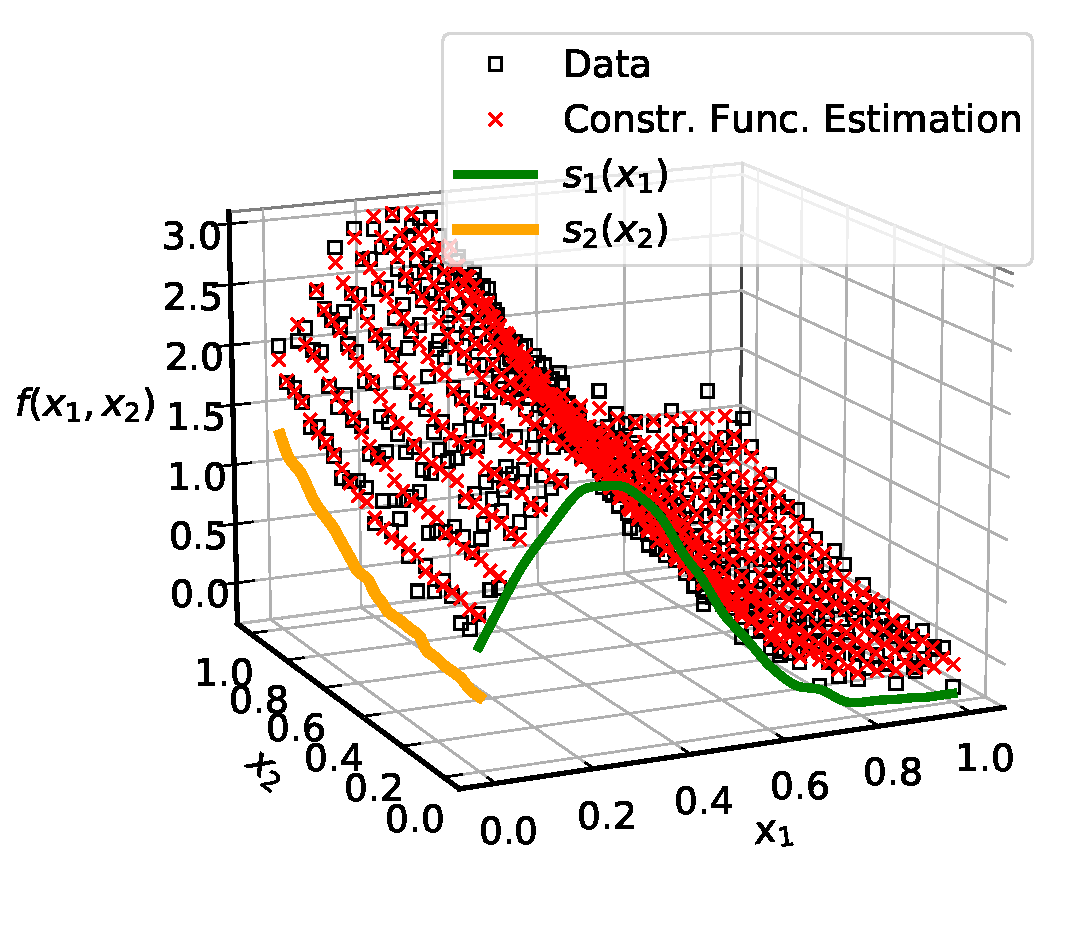
\includegraphics[width=\linewidth]{thesisplots/2d_example.pdf}
	\caption{2-d test function for n-d constrained function estimation}
	\label{fig:2d_example}
\end{figure}
